\documentclass [a4paper,12pt]{article}
\usepackage{url}
\usepackage{xcolor}
\usepackage{listings}
\usepackage{amssymb}
\usepackage{amsfonts}
\usepackage{graphicx}
\usepackage{caption}
\usepackage{subcaption}
\usepackage{units}
\usepackage{fullpage}


\definecolor{mygreen}{rgb}{0,0.6,0}
\definecolor{mygray}{rgb}{0.5,0.5,0.5}
\definecolor{mymauve}{rgb}{0.58,0,0.82}
\definecolor{mpi_green}{RGB}{27,92,40}

\lstset{ %
frame=single,
% xleftmargin=.05\textwidth, 
% xrightmargin=.05\textwidth,
%framexleftmargin=10pt,
rulecolor=\color{white},
backgroundcolor=\color{white},   % choose the background color; you must add \usepackage{color} or \usepackage{xcolor}
basicstyle=\ttfamily,        % the size of the fonts that are used for the code
breakatwhitespace=false,         % sets if automatic breaks should only happen at whitespace
breaklines=true,                 % sets automatic line breaking
captionpos=b,                    % sets the caption-position to bottom
commentstyle=\color{mygreen},    % comment style
deletekeywords={...},            % if you want to delete keywords from the given language
escapeinside={\%*}{*)},          % if you want to add LaTeX within your code
extendedchars=true,              % lets you use non-ASCII characters; for 8-bits encodings only, does not work with UTF-8
keepspaces=true,                 % keeps spaces in text, useful for keeping indentation of code (possibly needs columns=flexible)
keywordstyle=\color{mpi_green},       % keyword style
language=C++,                 % the language of the code
morekeywords={*,...},            % if you want to add more keywords to the set
numbers=left,                    % where to put the line-numbers; possible values are (none, left, right)
numbersep=5pt,                   % how far the line-numbers are from the code
numberstyle=\small\color{mygray}, % the style that is used for the line-numbers
rulecolor=\color{black},         % if not set, the frame-color may be changed on line-breaks within not-black text (e.g. comments (green here))
showspaces=false,                % show spaces everywhere adding particular underscores; it overrides 'showstringspaces'
showstringspaces=false,          % underline spaces within strings only
showtabs=false,                  % show tabs within strings adding particular underscores
stepnumber=1,                    % the step between two line-numbers. If it's 1, each line will be numbered
stringstyle=\color{mymauve},     % string literal style
tabsize=2%,                       % sets default tabsize to 2 spaces
%title=\lstname                   % show the filename of files included with \lstinputlisting; also try caption instead of title
}



\def \fftw {\texttt{fftw}}
\def \lmvn {\texttt{libmultiviewnative}}
\def \cufft {\texttt{cufft}}
\def \gpu {GPGPU}
\def \cpu {CPU}

\title{Streaming FFTs on large 3D microscope image data}
\author{Peter Steinbach, MPI CBG}
%\institute{MPI CBG}
\begin{document}
\maketitle
\begin{abstract}

\end{abstract}

\section{Introduction}

Light sheet microscopy today has become the hallmark experimental technique of systems biology \cite{Huisken13082004, Keller14112008}. It allows image aquisition of large alive developing specimens, high temporal and spatial resolution, imaging from multiple angles as well as low photodamage to the specimen which enables long timelapse recordings. However, due to the limited optical performance of the used equipment and the constant tradeoff between acquisition frequency and resolution, segmenting the produced data for further analysis is challenging. Deconvolution is the operation of restoring spatial resolution and contrast of this data given the knowledge of the underlying optics after the imagery has been recorded. Here, Selective Plane Illumination Microscopy (SPIM) data offers high potentials for SPIM records the same geometric location from different angles.\newline

The authors of \cite{2013arXiv1308.0730P} have provided an optimized formulation of the iterative expectation-maximization algorithm used to deconvolve SPIM data. This implementation thereof \cite{gh_spim_registration} is the starting point for this study whose motivation is to further increase performance and turnover of the algorithm by porting it entirely to run on General Purpose Graphics Processing Units (GPGPUs) using the CUDA programming platform \cite{Nickolls:2008:CUDA}. The implementation is available as a free and open-source library from \cite{lmvn_repo}.\newline

For the purpose of this paper, the subsequent discussion will first discuss the current algorithm implementation and common usage patterns(section \ref{sec:alg}), followed by a brief description of the benchmark hardware (section \ref{sec:hw}). The focus of the paper will then be on developing a performant implementation through a bottoms-up approach using model implementations (section \ref{sec:models}), before concluding with a summary and outlook (section \ref{sec:summ}).\newline

\section{Algorithm Details and Usage}
\label{sec:alg}
Given the recorded SPIM observations $\phi_\nu$ of a geometric volume for each angle $\nu$ (also referred to as \textit{view}), the current deconvolved estimate $\psi^{r+1}$ for iteration $r+1$ is given by (in a very general form):\newline

\begin{equation}
\psi^{r+1} = \psi^{r} \prod_{\nu \in V} \frac{\phi_{\nu}}{\psi^{r} \ast P_{\nu} } \ast P^{compound}_{\nu}
\label{iterative_deconv}
\end{equation}

Here, $P_{\nu}$ refers to the experimentally obtained optical point-spread function (PSF) for angle $\nu$. $\ast$ denotes the discrete convolution, i.e. given an image $f$ and a convolution kernel $g$ the convolution of the two would be given by $f \ast g$. $P^{compound}_{\nu}$ denotes a compound point spread function over virtual views calculated from all $P_{\nu}$. The interested reader is hereby referred to \cite{2013arXiv1308.0730P} for the derivation and further details that lead to and explain equation \ref{iterative_deconv}.\newline

The implementation of the above was performed in java \cite{fiji_wiki_mvd} and is available as a plugin to the fiji image analysis platform \cite{fiji_website}. The core algorithm can be described in pseudo-code as in listing \ref{lst:java_implementation}.\newline

\begin{lstlisting}[caption={Java Implementation of Multi-View Deconvolution.},label={lst:java_implementation}]
stack_f32 psi = stack_f32(const);
stack_f32 view[n_view], kernel1[n_view],     //loaded from disk
	  kernel2[n_view], weights[n_view];  //loaded from disk

for( i : n_iterations ){
  for( v : n_view ){
    stack_f32 temp = psi;
    temp = convolve(temp,kernel1[v]);	    
    temp = view[v]/temp;
    temp = convolve(temp,kernel2[v]);	    
    psi = regularize(psi, temp, weights);
  }
}
\end{lstlisting}

In listing \ref{lst:java_implementation}, \texttt{stack\_f32} refers to a type that describes a three dimensional image where each intensity is encoded as a 32-bit floating point number. Related to this, the C/C++ array notation is used to indicate that each run of the deconvolution requires all image views \texttt{stack\_f32 view[n\_view]}, all per-view PSFs \texttt{kernel1[n\_view]}, all compound PSFs \texttt{kernel2[n\_view]} and all weight distributions \texttt{weights[n\_view]} to be available in memory. \texttt{psi} notes the deconvolved view that is updated by each iteration of the double loop in line $4-5$. The function call \texttt{convolve} denotes the convolution described in equation \ref{iterative_deconv} as $\ast$. The regularization mentioned in listing \ref{lst:java_implementation} has been omitted from equation \ref{iterative_deconv} for the sake of clearity, but is further described in the corresponding paper \cite{2013arXiv1308.0730P}. Any padding to the input \texttt{view} and \texttt{weights} as well as embedding of both PSFs into zero-filled images of same shape as \texttt{view} is omitted from listing \ref{lst:java_implementation} for readability. \newline

%TODO add pictures of contrast improvement
% \begin{figure}[h]
%   \centering
%   \hfill
%   \begin{subfigure}[b]{0.45\textwidth}
%     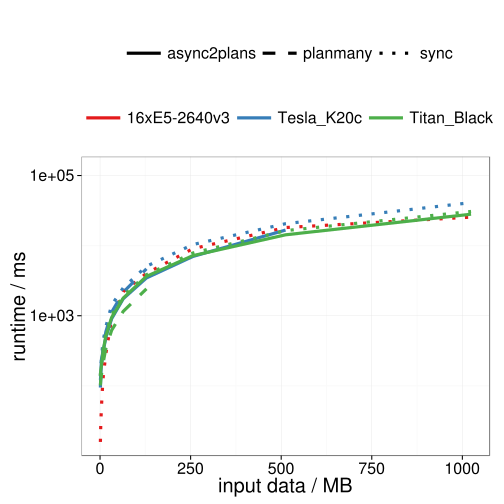
\includegraphics[width=\textwidth]{plots/batched_cgpu_runtime}
%     \caption{CUDA runtime}
%     \label{fig:batched_fft_runtime}
%   \end{subfigure}%
%   \hfill
%   \begin{subfigure}[b]{0.45\textwidth}
%     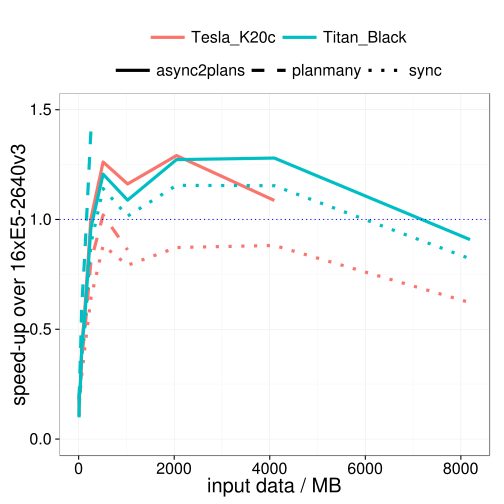
\includegraphics[width=\textwidth]{plots/batched_gpu_speed_up}
%     \caption{\gpu{} speed-up versus \cpu{}}
%     \label{fig:batched_fft_speed_up}
%   \end{subfigure}
%   \hfill
%   \caption{Runtimes for batched 3D FFT on synthetic data on \cpu{} with \fftw{} and on \gpu{} with \cufft{} (left, \ref{fig:single_fft_runtime}) and the relative speed-up of the asynchronous \gpu{} implementation using 2 streams (see figure \ref{fig:batched_fft_async2plans}) compared to the multi-core \cpu{} implementation (right, \ref{fig:batched_fft_speed_up})}
%   \label{fig:rt_batched_fft}
% \end{figure}


\begin{table}
  \begin{tabular}{ccc}                                                                                                                                                                              
    \hline                                                                                                                                                                                         
    View Shape  & Number of Views and Channels & Data Volume [MB]   \\
    \hline                                                       
    $928\times390\times390$ & $6 \times 1$ & $807$ \\
    $1670\times1070\times345$ & $4 \times 2$ & $4703$ \\
    \hline                                                                                                                                                                                         
  \end{tabular} 
  \label{typ_datasets}
  \caption{Typical SPIM datasets dimensionality, number of views and color channels (per view). All datasets save the pixel intensity as 16-bit integer value. The latter has been used to calculate the raw data set volume.}
\end{table} 

In order to set the implementation to scale, table \ref{typ_datasets} lists typical data sets from SPIM instruments. It is important to note that the majority of instruments store the image data as 16-bit integer value. Typical sizes of the PSF are on the order of $23 \times 81 \times 85$. \\

As the algorithm at hand relies twice on convolutions, this operation is deemed to be the largest consumer of run time. A convolution is a filtering operation, that operates on and n-dimensional image $f$ and convolves it by a filter kernel $g$ of similar or less dimensionality. Assuming that $f$ and $g$ are three-dimensional pixel collections and that $g$ has dimensions $N_{x} \times N_{y} \times N_{z}$, a convolution for an output pixel at location $[x,y,z]$ is calculated as 

\begin{equation}
  \label{eq:disc_convolve}
  (f \ast g)[x,y,z] = \sum^{i_x = N_{x}/2}_{i_x = -N_{x}/2} \sum^{i_y = N_{y}/2}_{i_y = -N_{y}/2} \sum^{i_z = N_{z}/2}_{i_z = -N_{z}/2} f[x-i_x,y-i_y,z-i_z] \cdot g[i_x,i_y,i_z].
\end{equation}

This operation does not only yield complications towards the borders of $f$ where $f[x-i_x,\dots]$ may refer to a pixel location outside the actual image (i.e. of unknown intensity), it is moreover of complexity 

\begin{equation}
\label{eq:discrete_convol_complexity}
\mathcal{O}(F[f \ast g]) = \mathcal{O}(I_{x} I_{y} I_{z} N_{x} N_{y} N_{z})
\end{equation}


where $I_{n}$ refers to the extent of $f$ in dimension $n$. Given the datasets listed in table \ref{typ_datasets}, this is an computationally expensive operation. As the convolution per output pixel $(f \ast g)[x,y,z]$ is independent of the calculation of every other output pixel $(f \ast g)[x',y',z']$, a convolution might at first glance yield high speed-ups when implemented on GPGPUs. As discussed in \cite{eklund_nonseparable_filtering}, this is only true for small kernel sizes on the order of $6 \times 6 \times 6$ at a fixed input image size. This is due to the fact that 2 arithmetic operations for every 2 arithmetic operations have to be performed. This results in an arithmetic complexity (number of arithmetic operations divided by the number of memory loads) of $1$. This has long been known \cite{massively_parallel_book} to be a regime, where GPGPUs do not perform well. To mitigate this short coming, the convolution theorem (equation \ref{}) can be exploited which states that a convolution in the spatial domain can be performed as a multiplication in the frequency domain.

\begin{equation}
  \label{eq:convol_theorem}
  F[f \ast g] = F[f] \cdot F[g]
\end{equation}

Here, $F[f]$ gives the Fourier Transform of $f$ into the frequency domain and $\cdot$ notes the element-wise multiplication of $F[f]$ and $F[g]$. The implementation of fast Fourier Transforms (FFT) has been studied for more than 50 years by now \cite{FFTCooleyTurkey,FFTBluestein,FFTRaders}. For the purpose of convolution, the complexity of the algorithm is hence reduced to 

\begin{equation}
  \label{eq:fft_convol_complexity}
  \mathcal{O}(F[f] \cdot F[g]) = 2\times\mathcal{O}(I\log I) + \mathcal{O}(I) = \mathcal{O}(I\log I)
\end{equation}

Here, $I = I_{x} \cdot I_{y} \cdot I_{z}$ refers to the total number of pixels in image $f$. As the FFT is performed on non-complex data further simplifications can be applied to it's implementation which renders equation \ref{eq:fft_convol_complexity} to be an upper bound rather than an exact value as in equation \ref{eq:discrete_convol_complexity}. The library as the result of the discussion at hand interfaces to the \texttt{fftw} (\cite{FFTW05}) library which contains highly optimised FFT implementations performed on the Central Processing Unit (CPU). The CPU-based implementation of the multi-view deconvolution is based on listing \ref{new_implementation}.

\begin{lstlisting}[caption={Optimized CPU Implementation of Multi-View Deconvolution. All FFT are explicitely stated \texttt{fft} as well as the corresponding normalized inverse operations \texttt{ifft}. },label={lst:new_implementation}]
stack_f32 psi = stack_f32(const);
stack_f32 view[n_view], kernel1[n_view],     //loaded from disk
	  kernel2[n_view], weights[n_view];  //loaded from disk

for( v : n_view ){
  kernel1[v] = fft(kernel1[v]);
  kernel2[v] = fft(kernel2[v]);
}

for( i : n_iterations ){
  for( v : n_view ){
    stack_f32 temp = psi;
    temp = ifft(fft(temp)*kernel1[v]);
    temp = view[v]/temp;
    temp = ifft(fft(temp)*kernel2[v]);
    psi = regularize(psi, temp, weights);
  }
}
\end{lstlisting}

Listing \ref{lst:new_implementation} contains one central improvement over listing \ref{lst:java_implementation}, whereby the FFT of \texttt{kernel1} and \texttt{kernel2} is performed before the iterative double loop is entered. This removes $n_{iterations}\cdot n_{view}$ executions of a FFT of size $I$ from the algorithm, which is beneficial not only in terms of runtime but also in terms of the memory budget.

For the GPGPU implementation interfacing to the \texttt{cufft} library (\cite{cufft}), the CPU implementation is used as a reference for code validation.


\clearpage
\section{Hardware}
\label{sec:hw}

For the measurements at hand, a Dell T7810 work station was used equipped with two Intel Xeon E5-2540 v3 processors and $\unit[64]{GB}$ of DDR4-2133 RAM. The workstation supported a Nvidia Tesla K20c provided by the TU Dresden based CUDA Center Of Excellence. The operating system was CentOS 7. To broaden the scope, a passively cooled Nvidia Tesla M2090 operated inside a rack-mounted Dell C6100 with two Intel Xeon E5-2640 and $\unit[128]{GB}$ of RAM. The operating system was CentOS 6.3 and all compilations were performed with gcc 4.8.3 and cuda 6.5. All compilations were performed with gcc 4.8.3 and cuda 6.5.14 except stated otherwise. Third, a second Dell T7810 work station with 2 Intel Xeon E5-2670 (Hyperthreading enabled), $\unit[64]{GB}$ of DDR4-2133 RAM and a Nvidia GeForce GTX Titan Black running CentOS 6.6 was included in the tests.

\section{Model}
\label{sec:models}

As shown in section \ref{sec:alg}, multi-view deconvolution relies on 3D image stack convolutions with large kernels. In order to iterate towards an efficient design of multi-view deconvolution, this section will discuss model implementations and their benchmarks on hardware introduced in section \ref{sec:hw}. All of the model systems use synthetic data which is validated after each run upon consistency where appropriate. If not stated otherwise, the synthetic data has been generated in steps of powers of 2 in each dimension, so that each benchmark was run on $64x64x64$, $128x64x64$, $128x128x64$, \dots, $1024x1024x1024$ shaped datasets if possible.

\subsection{Single FFT}

As the heart of the application are FFT, there performance on CPU and GPU should be compared. For this, the most simple setup is used.

\begin{lstlisting}[caption={Single FFT on synthetic data performed on CPU in pseudo-code based on the \fftw{} syntax.},label={lst:single_fft_cpu}]
stack_f32 synthetic_data;

fftwf_plan plan = fftw_plan_dft_r2c(3,
                                    synthetic_data.shape(),
                                    synthetic_data.ptr(),
                                    synthetic_data.ptr(),
                                    FFTW_MEASURE);
//start timing
fftwf_execute(plan)
//end timing
\end{lstlisting}

Listing \ref{lst:single_fft_cpu} gives an overview on the syntax required to execute a \fftw{} 3D FFT on spatial domain data and whose result is written back to the same memory location in the frequency domain (in-place transform). The application programming interface (API) requires plan to perform the transform operation. According to the documentation \cite{fftw_manual}, the plan allocates additional memory for structures required during FFT execution. This global variable hence exerts a software design force on all clients to be aware of this behavior. Moreover, plans should be reused in order to prevent unnecessary reallocations. The equivalent implementation to perform the FFT on the \gpu{} is given in listing \ref{lst:single_fft_gpu}.\newline

\begin{lstlisting}[caption={Single FFT on synthetic data performed on GPU in pseudo-code based on the \cufft{} syntax.},label={lst:single_fft_gpu}]
stack_f32 synthetic_data;
float* device_ptr = 0;
cudaMalloc(device_ptr, sizeof(float)*synthetic_data.size());
cudaMemcpy(device_ptr, synthetic_data.ptr() , sizeof(float)*synthetic_data.size(), cudaHostToDevice);

cufftHandle plan;
cufftPlan3d(&plan,synthetic_data.shape(0),synthetic_data.shape(1),synthetic_data.shape(2),CUFFT_R2C);

//start timing
cufftExecR2C(plan, device_ptr, device_ptr);
//end timing

cudaMemcpy(synthetic_data.ptr(), device_ptr , sizeof(float)*synthetic_data.size(), cudaDeviceToHost);
\end{lstlisting}

Clearly, the offload model of having \gpu{} memory being separate from \cpu{} memory requires a lot more syntax than for plain \cpu{} use cases. However, the \cufft{} API is similar in nature to \fftw{} except the more stringent procedural approach (no functions with return values, rather than functions operating on structs). As \texttt{cudaMemcpy} is used to transfer data from host to device and back, this implementation is internally synchronized.\newline

\begin{figure}[h]
  \centering
  \hfill
  \begin{subfigure}[b]{0.45\textwidth}
    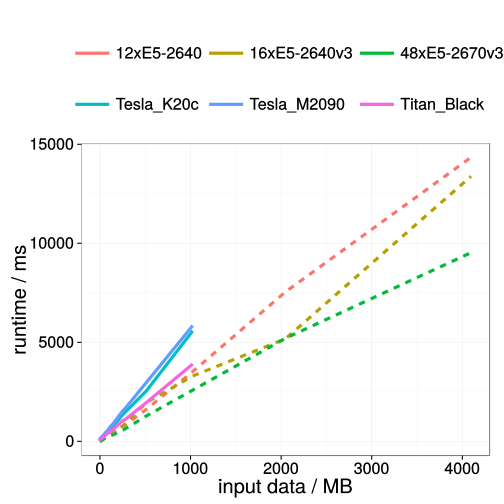
\includegraphics[width=\textwidth]{plots/synced_gpu_runtime}
    \caption{CUDA runtime}
    \label{fig:single_fft_runtime}
  \end{subfigure}%
  \hfill
  \begin{subfigure}[b]{0.45\textwidth}
    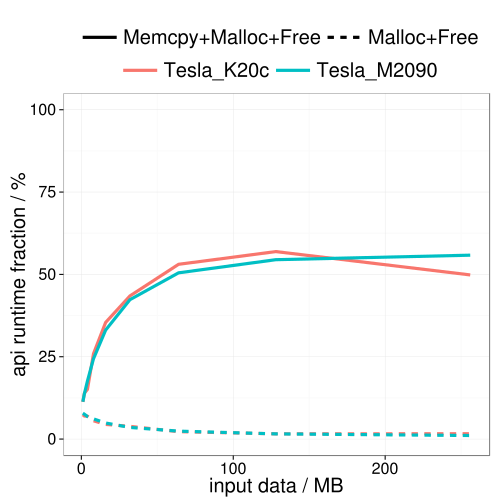
\includegraphics[width=\textwidth]{plots/synced_gpu_api_fractioninplace}
    \caption{CUDA API fraction}
    \label{fig:single_fft_api_fraction}
  \end{subfigure}
  \hfill
  \caption{Runtimes for single 3D FFT on synthetic data on \cpu{} with \fftw{} and on \gpu{} with \cufft{} (left, \ref{fig:single_fft_runtime}) and API time fraction of runtime dedicated to data (de-)allocation and/or data transfer (right, \ref{fig:single_fft_api_fraction}).}
  \label{fig:rt_single_fft}
\end{figure}

Figure \ref{fig:rt_single_fft} illustrates the runtime budget of an FFT transformation. Subfigure \ref{fig:single_fft_runtime} shows a linear rise in runtime with increasing input data. This is the behaviour expected from considerations of equation \ref{eq:fft_convol_complexity}. It is interesting to observed what fraction of this runtime is invested in data transfers. Figure \ref{fig:single_fft_api_fraction} hints to $\unit[50]{\%}$ of the total runtime is dedicated to data transfers. This implies, that if data transfer can be hidden or accelerated, this would beneficial for the entire algorithm.

\subsection{Batched FFTs}

\clearpage

\section{Summary}
\label{sec:summ}

Multiview Deconvolution is a central technique for contrast enhancements of multi-dimensional SPIM data. As the data is of unprecedented size, porting suche an algorithm onto massively parallel hardware (\gpu{}s) requires a constant struggle against data transfer bottlenecks. As such, the PCI Express is the everlasting hurdle to overcome by asynchronous orchestration of memory transfers to the \gpu{} and computing calls. In this study, performance considerations for model systems very similar to the environment of \lmvn{} lead to an improvement of the actual algorithm and a speed-up of $7x$ compared to a state-of-the-art multi-\cpu{} implementation.\newline


\section{Acknowledgements}
\label{sec:ackn}

I'd like to thank Stephan Preibisch (Janelia Farm) and Pavel Tomanck (MPI CBG) for providing me this challenging project that lead me to present at an internationally renowned conference. I'd also like to thank Stephan Janosch for providing test data sets and the CUDA Center of Excellence for providing the Nvidia Tesla K20c used for the experiments above as well as valuable feedback during this project. 

\section{References}
\bibliographystyle{ieeetr}
\bibliography{lmvn}
\end{document}
